\chapter{Datasets\label{sec:datasets}}\thispagestyle{empty}
\par{
    This thesis is based on five different existing publically available datasets.
    This chapter discusses these datasets based on different criteria: \newline
    \textbf{Source:} reference of the owner of the dataset and brief description of the original purpose of the dataset.\newline
    \textbf{Patient sample:} statistics of the patients whose medical images were collected such as age, gender and possible spine pathologies.\newline
    \textbf{Technical information:} discusses the imaging technology, the image resolution and the spatial dimensions of the image. 
}
\section{Dataset overview}
\par{
    Table \ref{tab:datasetReferences} provides an overview of the 5 datasets sourced for this work.
    This table shows there are important differences between the datasets in imaging mode and dataset size.
    Figure \ref{fig:AllDataset_dims} also indicates the differences in image dimensions and resolutions.
    For more details on the data quantity, please consult chapter \ref{seg:datasetcomparison}. 
    Notably, the fact that some images were taken from the same patient is vital to recognize. It means the dataset is grouped. 
}
\begin{SCtable}[\sidecaptionrelwidth][h]
 
    \begin{tabular}{ l l l l l} 
     \toprule
     Name & reference & imaging & Quantity & Annotation \\
          &           & technology & [images] & \\
     \hline 
    UWSpine & \cite{Glocker}  & \acrshort{ct} & 125 & point  \\ 
    xVertSeg & \cite{Ibragimov2014, Korez2015} & \acrshort{ct} & 15 & full \\
    UniSiegen  & \cite{Zukic2014} & \acrshort{mri} & 17 & full \\
    PLoS & \cite{Chu2015} & \acrshort{mri} & 23 & semantic \\
    MyoSegmenTUM & \cite{Burian2019} & \acrshort{mri} &  54 & full \\
     \bottomrule
    \end{tabular}
    \caption{List of dataset references. 
    The agreement with prof. T. Vrtovec regarding the xVertSeg dataset can be found in appendix \ref{seg:datasetagreement}.\label{tab:datasetReferences}}

\end{SCtable}
\par{
    In table \ref{tab:dataOrientation} illustrates the difference in anatomical orientation of the volumes in the different datasets.
    To execute the modelling approach discussed in chapter \ref{sec:model_concept}, all volume orientations were uniformized to assure that for all datasets, the volume slices along dimension 0 represent the transverse slices, 
    the slices along dimension 1 represent the frontal slices, and the slices along dimension 2 are sagittal plane coupes of the volume.
}
\begin{SCtable}[\sidecaptionrelwidth][h]
 
    \begin{tabular}{ l l l l} 
     \toprule
     Name & X & Y & Z \\
     \hline 
    UWSpine & Left-right & Anteroposterior & Craniocaudal \\
    xVertSeg & Left-right & Anteroposterior & Craniocaudal \\
    UniSiegen  &  Anteroposterior & Craniocaudal & Left-right \\
    PLoS & Left-right & Anteroposterior & Craniocaudal$^\dagger$ \\
    MyoSegmenTUM &  Anteroposterior & Craniocaudal & Left-right \\
     \bottomrule
    \end{tabular}
    \caption{List of dataset orientations. Clarification of the names of the anatomical axis is given in figure \ref{fig:anatomicalPlains}.
    The names of the axis, $X$, $Y$ and $Z$ represent the \texttt{numpy} axis \texttt{0}, \texttt{1} and \texttt{2}.
    $^\dagger$ The Craniocaudal axis in the PLoS dataset is inverted.\label{tab:dataOrientation}
    }
\end{SCtable}
\begin{SCfigure}[][htb]
    \centering
    \begin{minipage}{.4\textwidth}
        \includegraphics[width=.98\textwidth]{automated_graphs/AllDataset_DimensionsBoxplot.png}
    \end{minipage}%
    \begin{minipage}{0.4\textwidth}
        \includegraphics[width=.98\textwidth]{automated_graphs/AllDataset_SpacingBoxplot.png}
    \end{minipage}
    \caption{Boxplots comparing the scan dimensions and initial resolution of the different datasets.
    The left column indicates the volume dimensions (in mm) in the different datasets. 
    The graphs indicate there are important differences between the datasets. Notice that both the USiegen and the MyoSegmenTUM dataset are cropped severely in the left-right direction.
    The right column represents the vixel spacings in the different volumes of the different datasets.
    In the preprocessing step all volumes are resampled on a $1mm \times 1mm \times 1mm$ grid, see page \pageref{sec:resampling}. \label{fig:AllDataset_dims} 
    }
\end{SCfigure}
\FloatBarrier
\begin{SCfigure}[][htb]
    \centering
    \includegraphics[width=10cm]{/home/thesis/images/Anatomical_Planes.png}
    \caption{\label{fig:anatomicalPlains}Clarification of the anatomical planes. 
    For some images further in this document, for example figure \ref{fig:comb1_1} at page \pageref{fig:comb1_1}, the anatomical axes will be referred to by numbering:
    Slices perpendicular to dimension 0 are slices in the transverse plane.
    Slices perpendicular to dimension 1 are slices in the frontal plane.
    Slices perpendicular to dimension 2 are slices in the sagittal plane.  
    }
\end{SCfigure}
\section{Comparison of the different datasets\label{seg:datasetcomparison}}
\subsection{xVertSeg\label{sec:xVertSeg}}



The xVertSeg \cite{Ibragimov2014, Korez2015} was kindly made available by prof. T. Vrtovec (University of Ljubljana, Faculty of Electrical Engineering, Slovenia), see appendix \ref{seg:datasetagreement} for the agreement.
This dataset contains 25 \acrfull{ct} scans of the lumbar spine, of which 15 \acrshort{ct} scans are fully labeled.
Given the provided metadata\footnote{patient age and gender.}, it is clear these 15 scans were collected from 15 different patients.

For each of these 15 scans, full instance segmentation masks for all 5 lumbar vertebrae are provided. The delineation was performed by a skilled professional.

Additionally, for each vertebra a fracture class and fracture grade is provided. 
Apart from vertebrae classified as \textit{normal}, the dataset contains \textit{mild}, \textit{moderate} and \textit{severe} cases of vertebrae fracture types \textit{wedge}, \textit{crush} and \textit{biconcavity}.
\marginpar{
        % This file was created by tikzplotlib v0.9.8.
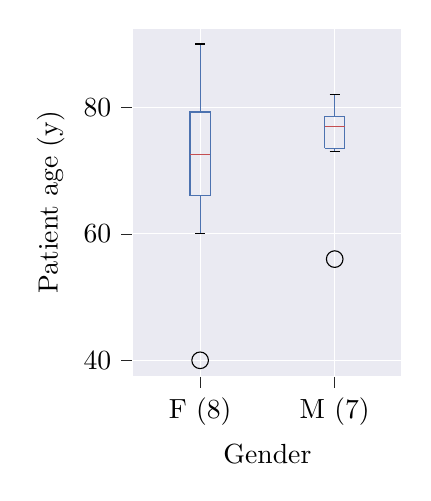
\begin{tikzpicture}

\definecolor{color0}{rgb}{0.917647058823529,0.917647058823529,0.949019607843137}
\definecolor{color1}{rgb}{0.298039215686275,0.447058823529412,0.690196078431373}
\definecolor{color2}{rgb}{0.768627450980392,0.305882352941176,0.32156862745098}

\begin{axis}[
axis background/.style={fill=color0},
axis line style={white},
height=6cm,
tick align=outside,
tick pos=left,
width=5cm,
x grid style={white},
xlabel={Gender},
xmajorgrids,
xmin=0.5, xmax=2.5,
xtick style={color=white!15!black},
xtick={1,2},
xticklabels={F (8),M (7)},
y grid style={white},
ylabel={Patient age (y)},
ymajorgrids,
ymin=37.5, ymax=92.5,
ytick style={color=white!15!black}
]
\addplot [color1, opacity=1]
table {%
0.925 66
1.075 66
1.075 79.25
0.925 79.25
0.925 66
};
\addplot [color1, opacity=1]
table {%
1 66
1 60
};
\addplot [color1, opacity=1]
table {%
1 79.25
1 90
};
\addplot [black, opacity=1]
table {%
0.9625 60
1.0375 60
};
\addplot [black, opacity=1]
table {%
0.9625 90
1.0375 90
};
\addplot [black, mark=o, mark size=3, mark options={solid,fill opacity=0}, only marks]
table {%
1 40
};
\addplot [color1, opacity=1]
table {%
1.925 73.5
2.075 73.5
2.075 78.5
1.925 78.5
1.925 73.5
};
\addplot [color1, opacity=1]
table {%
2 73.5
2 73
};
\addplot [color1, opacity=1]
table {%
2 78.5
2 82
};
\addplot [black, opacity=1]
table {%
1.9625 73
2.0375 73
};
\addplot [black, opacity=1]
table {%
1.9625 82
2.0375 82
};
\addplot [black, mark=o, mark size=3, mark options={solid,fill opacity=0}, only marks]
table {%
2 56
};
\addplot [color2, opacity=1]
table {%
0.925 72.5
1.075 72.5
};
\addplot [color2, opacity=1]
table {%
1.925 77
2.075 77
};
\end{axis}

\end{tikzpicture}

        \captionof{figure}{xVertSeg patients age distribution}
        \label{fig:xVertSeg_Age}
    }

\subsubsection{Original Objective of the Dataset}

The dataset was collected for the \textit{xVertSeg challenge}\footnote{see \url{http://lit.fe.uni-lj.si/xVertSeg/database.php}, this challenge was organized by the University of Ljubljana in 2015}.
Based on the 15 provided scans with corresponding masks, the participants were required to construct a model to make predictions on the test set of 10 unlabelled scans.

The challenge consisted of two tasks:
\begin{enumerate}
    \item Segmentation of the lumbar vertebrae. For each scan in the test set, the segmentation masks of the lumbar vertebrae were requested.
    \item Fracture classification on the segmented vertebrae, consisting of morphological grade and fracture classification.
\end{enumerate}

\subsubsection{Patient statistics}

The patients in the xVertSeg dataset train set consist of 8 females and 7 males.
The age of these patients is slightly higher than for the other datasets.
The average patient in this dataset is 71 years old.
A box plot of the age distribution between genders is shown in figure \ref{fig:xVertSeg_Age}. 

\begin{SCtable}[\sidecaptionrelwidth][h]
    \centering
        \begin{tabular}{lrrrrrr}
\toprule
{} &  L1 &  L2 &  L3 &  L4 &  L5 &  Total \\
\midrule
biconcave &   6 &   7 &   8 &   4 &   2 &     27 \\
normal    &   5 &   6 &   4 &   4 &   7 &     26 \\
wedge     &   3 &   2 &   2 &   3 &   2 &     12 \\
crush     &   1 &   0 &   1 &   4 &   4 &     10 \\
\bottomrule
\end{tabular}

        \caption{Every patient in the xVertSeg dataset suffers from at least one spine pathology.
        Most of these pathologies are identified as \textit{mild}.
        This table counts the spine pathologies and normal vertebrae observed over all 15 patients in the xVertSeg dataset.}   
\end{SCtable}

\subsubsection{Technical information}

The xVertSeg dataset contains 15 \acrshort{ct} annotated scans. 
On figure \ref{fig:xVertSeg_image002}, two slices of the same patient (002) are represented.
The slices show the complete, uncropped sections of the torso and abdominal region of the patient. 
There is no \acrshort{roi} cropping in the transverse plane.
The average left-right axis span of the volumes is 417 mm. Along the anteroposterior direction, this is 421 mm. 
Along the craniocaudal axis, the volumes are cropped. The average volume extend in this direction is 279 mm.

\begin{SCfigure}[][htb]
    \centering
    \includegraphics[width=.95\textwidth]{automated_graphs/xVertSeg_image002.png}
    \caption{xVertSeg scan \textit{image002}. \label{fig:xVertSeg_image002}. In the xVertSeg dataset, the volume left-right axis is not cropped. These images only show part of the sacrum, but multiple thoricic vertebrae are visible.}
\end{SCfigure}

The distribution of the scan dimensions is shown in figure \ref{fig:AllDataset_dims}. This also illustrates that the \textit{xVertSeg} dataset consists of large, high-resolution images.
Mind that during pre-processing, the scans are resampled on a $1mm \times 1mm \times 1mm$ grid.
\FloatBarrier

\subsection{UniSiegen}

This dataset is made available by the University of Siegen, Germany.
It was constructed by dr. D. Zukic \cite{Zukic2014} as part of his PhD project.

This dataset contains 17 \acrshort{mri} scans of xxx patients

The dataset con

\subsubsection{Original Objective of the Dataset}

This dataset was 

\subsubsection{Patient statistics}

\marginpar{
        % This file was created by tikzplotlib v0.9.8.
\begin{tikzpicture}

\definecolor{color0}{rgb}{0.917647058823529,0.917647058823529,0.949019607843137}
\definecolor{color1}{rgb}{0.298039215686275,0.447058823529412,0.690196078431373}
\definecolor{color2}{rgb}{0.768627450980392,0.305882352941176,0.32156862745098}

\begin{axis}[
axis background/.style={fill=color0},
axis line style={white},
tick align=outside,
tick pos=left,
x grid style={white},
xlabel={Gender},
xmajorgrids,
xmin=0.5, xmax=2.5,
xtick style={color=white!15!black},
xtick={1,2},
xticklabels={Female (11 patients),Male (6 patients)},
y grid style={white},
ylabel={Patient age (y)},
ymajorgrids,
ymin=18.35, ymax=76.65,
ytick style={color=white!15!black}
]
\addplot [color1, opacity=1]
table {%
0.925 21.5
1.075 21.5
1.075 38.5
0.925 38.5
0.925 21.5
};
\addplot [color1, opacity=1]
table {%
1 21.5
1 21
};
\addplot [color1, opacity=1]
table {%
1 38.5
1 55
};
\addplot [black, opacity=1]
table {%
0.9625 21
1.0375 21
};
\addplot [black, opacity=1]
table {%
0.9625 55
1.0375 55
};
\addplot [black, mark=o, mark size=3, mark options={solid,fill opacity=0}, only marks]
table {%
1 74
1 69
};
\addplot [color1, opacity=1]
table {%
1.925 33
2.075 33
2.075 69.5
1.925 69.5
1.925 33
};
\addplot [color1, opacity=1]
table {%
2 33
2 27
};
\addplot [color1, opacity=1]
table {%
2 69.5
2 72
};
\addplot [black, opacity=1]
table {%
1.9625 27
2.0375 27
};
\addplot [black, opacity=1]
table {%
1.9625 72
2.0375 72
};
\addplot [color2, opacity=1]
table {%
0.925 22
1.075 22
};
\addplot [color2, opacity=1]
table {%
1.925 58
2.075 58
};
\end{axis}

\draw ({$(current bounding box.south west)!0.5!(current bounding box.south east)$}|-{$(current bounding box.south west)!0.98!(current bounding box.north west)$}) node[
  scale=0.6,
  anchor=north,
  text=white!15!black,
  rotate=0.0,
  align=center
]{USiegen dataset
age distribution};
\end{tikzpicture}

        \captionof{figure}{Distribution of patient age in the USiegen dataset.}
        \label{fig:xVertSeg_Transverse}
    }


\subsubsection{Technical information}



\FloatBarrier
\subsection{PLos}

\subsubsection{Patient statistics}

\subsubsection{Technical information}

\subsubsection{Original Objective of the Dataset}
\FloatBarrier
\subsection{MyoSegmenTUM datset}

This dataset is made available by S. Schläger from the Technische Universität München via the \acrfull{osf} \footnote{see \url{ https://osf.io/3j54b/?view_only=f5089274d4a449cda2fef1d2df0ecc56 }}.
It was constructed for the MyoSegmenTUM project \cite{Durian2019}.
It consists of 53 \acrshort{mri} scans of the spine.

\subsubsection{Original Objective of the Dataset}

The MyoSegmenTUM Spine dataset is compiled as a reference dataset for development of segmentation algorithms of the lumbar spine vertebral bodies and  muscle groups.

\subsubsection{Patient statistics}

In figure \ref{fig:OSF_ageboxplot}, the age distribution of the patients in the MyoSegmenTUM dataset is shown.

\marginpar{
        % This file was created by tikzplotlib v0.9.8.
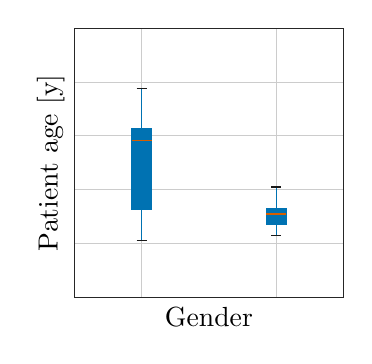
\begin{tikzpicture}

\definecolor{color0}{rgb}{0,0.447058823529412,0.698039215686274}
\definecolor{color1}{rgb}{0.835294117647059,0.368627450980392,0}

\begin{axis}[
axis line style={white!15!black},
height=5cm,
tick align=outside,
width=5cm,
x grid style={white!80!black},
xlabel={Gender},
xmajorgrids,
xmajorticks=false,
xmin=0.5, xmax=2.5,
xtick style={color=white!15!black},
xtick={1,2},
xticklabels={F(39),M(15)},
y grid style={white!80!black},
ylabel={Patient age [y]},
ymajorgrids,
ymajorticks=false,
ymin=0, ymax=100,
ytick style={color=white!15!black}
]
\addplot [color0, opacity=1]
table {%
1 32.5
1 21
};
\addplot [color0, opacity=1]
table {%
1 62.7652292950034
1 77.6673511293635
};
\addplot [white!10!black, opacity=1]
table {%
0.9625 21
1.0375 21
};
\addplot [white!10!black, opacity=1]
table {%
0.9625 77.6673511293635
1.0375 77.6673511293635
};
\addplot [color0, opacity=1]
table {%
2 27
2 23
};
\addplot [color0, opacity=1]
table {%
2 33
2 41
};
\addplot [white!10!black, opacity=1]
table {%
1.9625 23
2.0375 23
};
\addplot [white!10!black, opacity=1]
table {%
1.9625 41
2.0375 41
};
\path [draw=color0, fill=color0]
(axis cs:0.925,32.5)
--(axis cs:1.075,32.5)
--(axis cs:1.075,62.7652292950034)
--(axis cs:0.925,62.7652292950034)
--(axis cs:0.925,32.5)
--cycle;
\path [draw=color0, fill=color0]
(axis cs:1.925,27)
--(axis cs:2.075,27)
--(axis cs:2.075,33)
--(axis cs:1.925,33)
--(axis cs:1.925,27)
--cycle;
\addplot [color1, opacity=1]
table {%
0.925 58.2888432580424
1.075 58.2888432580424
};
\addplot [color1, opacity=1]
table {%
1.925 31
2.075 31
};
\end{axis}

\end{tikzpicture}

        \captionof{figure}{Distribution of patient age in the dataset from the MyoSegmenTUM project.}
        \label{fig:OSF_ageboxplot}
    }



\subsubsection{Technical information}

\begin{SCfigure}[][htb]
    \centering
    \includegraphics[width=.95\textwidth]{automated_graphs/OSF_02.png}
    \caption{MyoSegmenTUM dataset scan \textit{02}. \label{fig:OSF_02}}
\end{SCfigure}
\FloatBarrier
\subsection{UWSpine}

This dataset is made available by the University of Washington.
It has been constructed by dr. Glocker and team \cite{Glocker2012,Glocker2013}.

This dataset contains 242 \acrshort{ct} scans of 150 different patients.
This grouped nature of the data will be taken into account when performing the train-validation-test split.

\subsubsection{Original Objective of the Dataset}

\subsubsection{Patient statistics}

\marginpar{
        % This file was created by tikzplotlib v0.9.8.
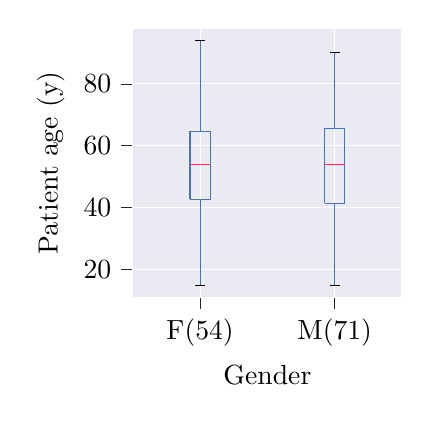
\begin{tikzpicture}

\definecolor{color0}{rgb}{0.917647058823529,0.917647058823529,0.949019607843137}
\definecolor{color1}{rgb}{0.298039215686275,0.447058823529412,0.690196078431373}
\definecolor{color2}{rgb}{0.768627450980392,0.305882352941176,0.32156862745098}

\begin{axis}[
axis background/.style={fill=color0},
axis line style={white},
height=5cm,
tick align=outside,
tick pos=left,
width=5cm,
x grid style={white},
xlabel={Gender},
xmajorgrids,
xmin=0.5, xmax=2.5,
xtick style={color=white!15!black},
xtick={1,2},
xticklabels={F(54),M(71)},
y grid style={white},
ylabel={Patient age (y)},
ymajorgrids,
ymin=11.05, ymax=97.95,
ytick style={color=white!15!black}
]
\addplot [color1, opacity=1]
table {%
0.925 42.75
1.075 42.75
1.075 64.75
0.925 64.75
0.925 42.75
};
\addplot [color1, opacity=1]
table {%
1 42.75
1 15
};
\addplot [color1, opacity=1]
table {%
1 64.75
1 94
};
\addplot [black, opacity=1]
table {%
0.9625 15
1.0375 15
};
\addplot [black, opacity=1]
table {%
0.9625 94
1.0375 94
};
\addplot [color1, opacity=1]
table {%
1.925 41.5
2.075 41.5
2.075 65.5
1.925 65.5
1.925 41.5
};
\addplot [color1, opacity=1]
table {%
2 41.5
2 15
};
\addplot [color1, opacity=1]
table {%
2 65.5
2 90
};
\addplot [black, opacity=1]
table {%
1.9625 15
2.0375 15
};
\addplot [black, opacity=1]
table {%
1.9625 90
2.0375 90
};
\addplot [color2, opacity=1]
table {%
0.925 54
1.075 54
};
\addplot [color2, opacity=1]
table {%
1.925 54
2.075 54
};
\end{axis}

\end{tikzpicture}

        \captionof{figure}{Distribution of patient age in the dataset from Washington University.}
        \label{fig:xVertSeg_Transverse}
    }



\subsubsection{Technical information}

\section{Train, validation and test split considerations\label{sec:trainValTestSplit}}

To allow evaluation of the models produced, a test set is split from the development set.
The objective is to evaluate how well a model generalizes to new data\footnote{
    New data is to be interpreted here as a new sample from \textit{the same population} as the development sample.
    Unfortunately, it cannot be claimed that the different datasets I collected indeed form a perfect representation of the population of medical images of the lumbar spine.}. 
To provide an honest estimate of the out-of-sample performance, the test dataset should represent the investigated population and (hidden) correlations with elements of the development sample should be avoided.

This is done\footnote{
    To accomplish this, I used the function \texttt{GroupedStratifiedSplit} at \url{https://github.com/scikit-learn/scikit-learn/pull/18649/}. 
    This class is not yet part of the official \texttt{sci-kit learn} library release (at the time of writing) but functions well for this application.} taking into account the following:
\begin{description}
    \item[Stratified data:] The combination of data from different sources is stratified. Every source is considered a subpopulation. The data split is made such that the proportion of scans originating from each data source in every split is proportional to their occurrence in the total population.
    \item[Grouped data:] The scans of the same patient can be assumed to be correlated to each other. These scans should not be spread over different splits. The data is split at patient level.
\end{description}

For each datasource, the intended split is $\frac{4}{6}$ for train set, $\frac{1}{6}$ for cross validation set and $\frac{1}{6}$ for test set.
This distribution is not perfect but acceptable, as is indicated by the values in table \ref{tab:summary_split}.

\begin{SCtable}[\sidecaptionrelwidth][h]
 
    \begin{tabular}{lrrr}
\toprule
split &  test &  train &  xval \\
source       &       &        &       \\
\midrule
MyoSegmenTUM &     9 &     33 &     9 \\
PLoS         &     4 &     14 &     4 \\
USiegen      &     2 &     14 &     1 \\
xVertSeg     &     2 &     10 &     3 \\
\bottomrule
\end{tabular}

    \caption{Number of volumes by datasource and by split. The scan volumes are split such that scans of the same patient are in the same split set.\label{tab:summary_split}}
  
  \end{SCtable}

  \begin{SCtable}[\sidecaptionrelwidth][h]
 
    \begin{tabular}{ll|lll|l}
    \toprule
    split        &            & test & train & xval & total \\
    source       & dimension  &      &       &      &       \\ \hline
    MyoSegmenTUM & Transverse & 1989 & 7293  & 1989 & 11271 \\
                 & Frontal    & 1989 & 7293  & 1989 & 11271 \\
                 & Sagittal   & 720  & 2650  & 725  & 4095  \\
    PLoS         & Transverse & 1528 & 5348  & 1528 & 8404  \\
    USiegen      & Transverse & 733  & 5063  & 501  & 6297  \\
                 & Frontal    & 681  & 4276  & 1080 & 6037  \\
                 & Sagittal   & 145  & 1089  & 180  & 1414  \\
    xVertSeg     & Transverse & 759  & 2652  & 785  & 4196  \\
                 & Frontal    & 812  & 4163  & 1290 & 6265  \\
                 & Sagittal   & 812  & 4163  & 1290 & 6265  \\ \hline
    total        & Transvers  & 5009 & 20356 & 4803 & 30168 \\
                 & Frontal    & 3482 & 15732 & 4359 & 23573 \\
                 & Sagittal   & 1677 & 7902  & 2195 & 11774 \\ \bottomrule
    \end{tabular}
    \caption{Number of slices by data source and by split.
    These values might seem high, yet, the reader should not forget that these image slices are highly correlated. 
    There is very little additional independent information comparing one slice with a slice taken just 1mm further.
    On top of this, many slices only contain the background class without providing the model information to train on the lumbar vertebrae classes. 
    \label{tab:summary_split_slices}}
  
  \end{SCtable}

